\chapter{Evaluation and Results comparison}
\label{chapter:evaluation}

In the previous chapters the description of the methods and of the key sections of the designed algorithms has been carried out.
In Chapter~\ref{chapter:methods} a general outline of the implemented idea has been presented.
Instead, Chapter~\ref{chapter:implementation} illustrates the key functions and the computations that build up the entire algorithm.\\
\textbf{Probably in the previous chapter it would be good to put some pseudocode (for example for the main parts) in order to give not only a qualitative description of the algorithm but highlight the main functions}.\\
Therefore, the functions exploited in the pre and post-processing phases have been previously outlined. 
Moreover, the two novel strategies designed have been reported, underlining the procedure implemented for obtaining the estimations of the grid points, the matching cost methods tested and their efficiency throughout the algorithm and the correlation with previously created stereo matching algorithms. 
Chapter~\ref{chapter:methods} contains also a brief presentation of similar ideas developed in standard and in deep learning based methods, which were exploited to obtain an initial proof of the potential performance of the algorithm.\\
Thus, this chapter delineates the results obtained supporting the discussion with images of the point cloud and the disparity maps obtained.
Moreover, some general comments related to the different result are going to be presented.
In fact, a discussion focused on the considerations that can be carried out from the outcomes obtained will cover Chapter~\ref{chapter:discussion}.\\
Here the interest is centred on the results achieved and in the comparison between the OpenCV method, defined as the baseline, and the algorithms designed.
Moreover, in the first part of the following analysis the outcomes collected during the initial phase of the whole work are proposed.
As previously introduced, their main function was to provide, at the beginning of the developed project, a proof of the feasibility of the thought strategy. 
That was, in fact, extremely useful for having, from the very beginning, a qualitative guidance on the project development. 

\section{Researching phase results}
\label{section:research-phase-results}

\begin{figure}[t]
	\centering
	\subfigure[Left RGB test image]{
 		\includegraphics[width=0.4\textwidth, height= 5cm, keepaspectratio]{images/left-playtable-test.png}
 		\label{fig:test-matlab-left-02}
}
	\subfigure[Right RGB test image]{
 		 \includegraphics[width=0.4\textwidth, height= 5cm, keepaspectratio]{images/right-playtable-test.png}
 		 \label{fig:test-matlab-right-02}
}
	\subfigure[Disparity test image]{
	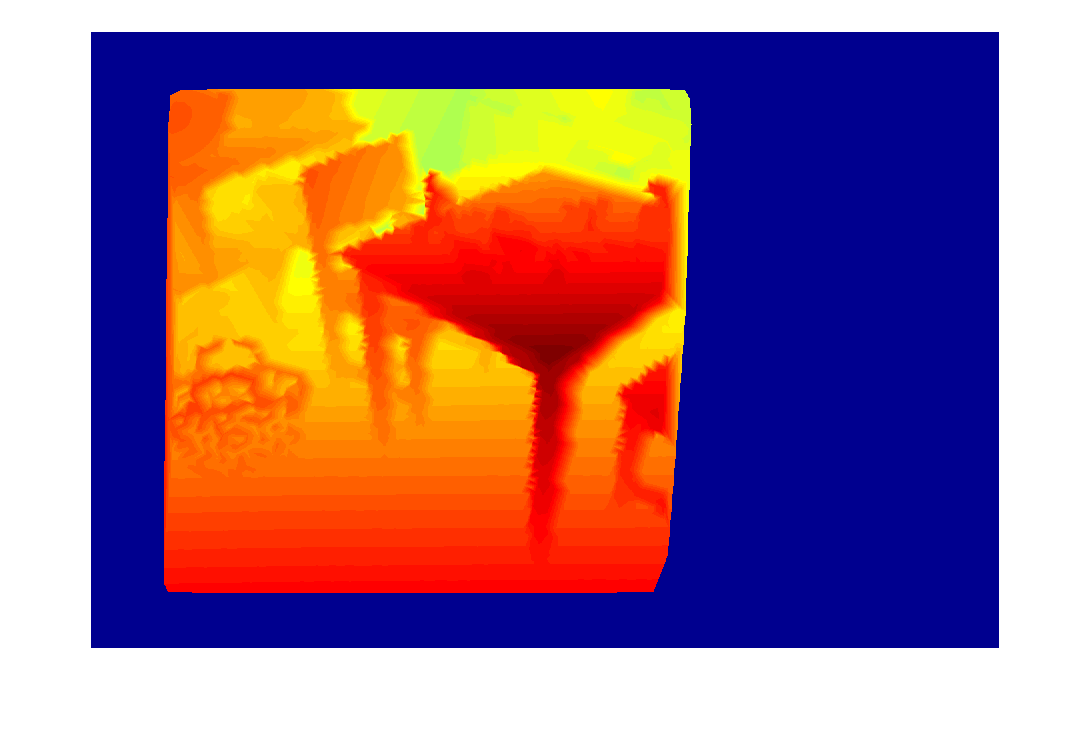
\includegraphics[width=0.8\textwidth, height=5cm, keepaspectratio]{images/disparity-map-playtable-test.png}
	\label{fig:disparity-test-02}
}
\caption{Test images from the Middlebury 2014 dataset with disparity image estimated with linear simple semi-global matching based method to test feasibility of thought strategy}
\label{fig:test-matlab-02}
\end{figure}

Figure~\ref{fig:test-matlab-02} displays the result of the estimation of a disparity image exploiting a stereo pair from the Middlebury 2014 dataset.
The disparity map shown in Figure~\ref{fig:disparity-test-02} has been achieved applying a rather simple and linear implementation of a semi-global based method, where information from an initial simulated sparse grid of point is employed.
As a matter of fact, in that initial stage of the project designing, the overall performance was not taken into account.
The main focus was the feasibility of the procedure compared to standard SGM-based algorithms. 
In fact, the core of the algorithm computations stand in the matching cost phase, which is based on the Center-Symmetric Census transform and on the Hamming distance computation.
Then, the aggregation cost step is carried out only over the four main orthogonal directions.
Finally, a basic left-right consistency check procedure is applied, which generate the lost of information of the two image sides.
Clearly, this behaviour is related to the disparity range employed in the algorithm.

\section{Derivative method results}
\label{section:der-method-results}

\begin{figure}[t]
	\centering
	\subfigure[Derivative-based method]{
 		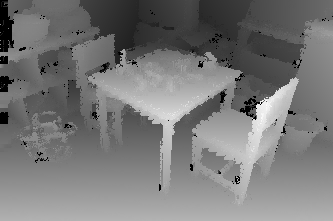
\includegraphics[width=0.4\textwidth, height= 5cm, keepaspectratio]{images/raw-disparity-playtable-test.png}
 		\label{fig:derivative-based-test-table}
}
	\subfigure[SGM-based method]{
 		 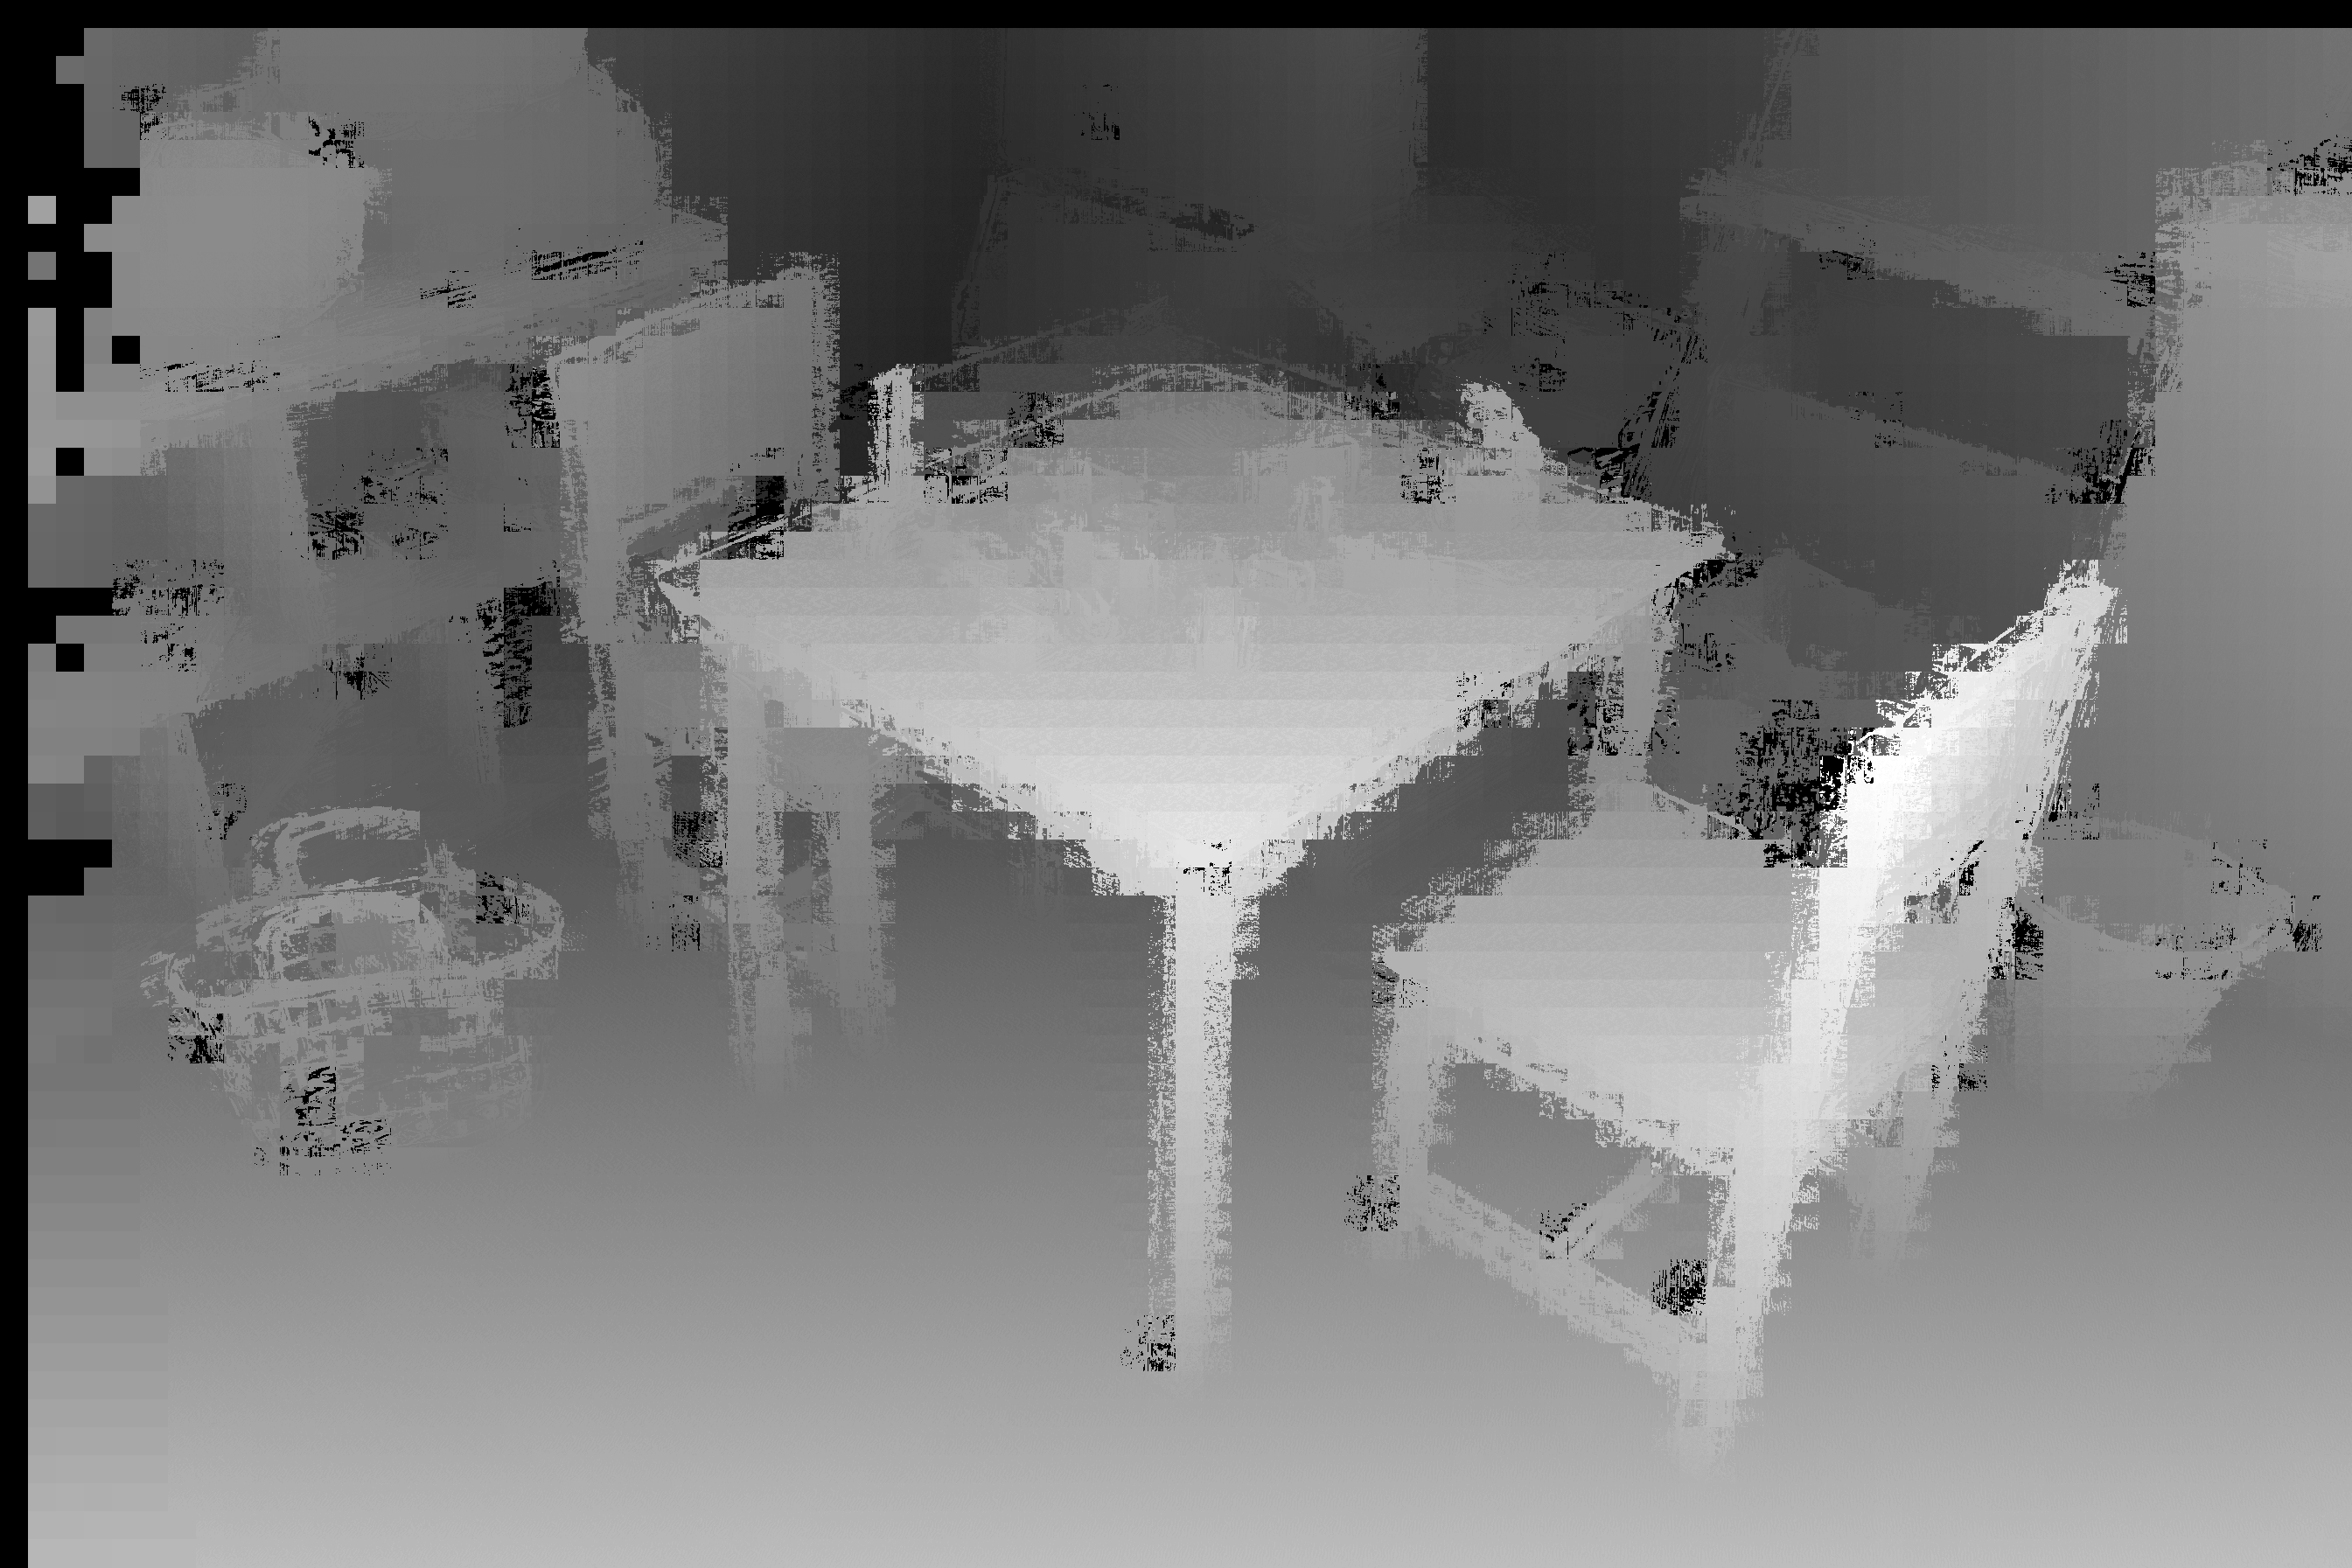
\includegraphics[width=0.4\textwidth, height= 5cm, keepaspectratio]{images/sgm-based-playtable-test.png}
 		 \label{fig:sgm-based-test-table}
}
	\subfigure[OpenCV stereoSGBM method]{
	 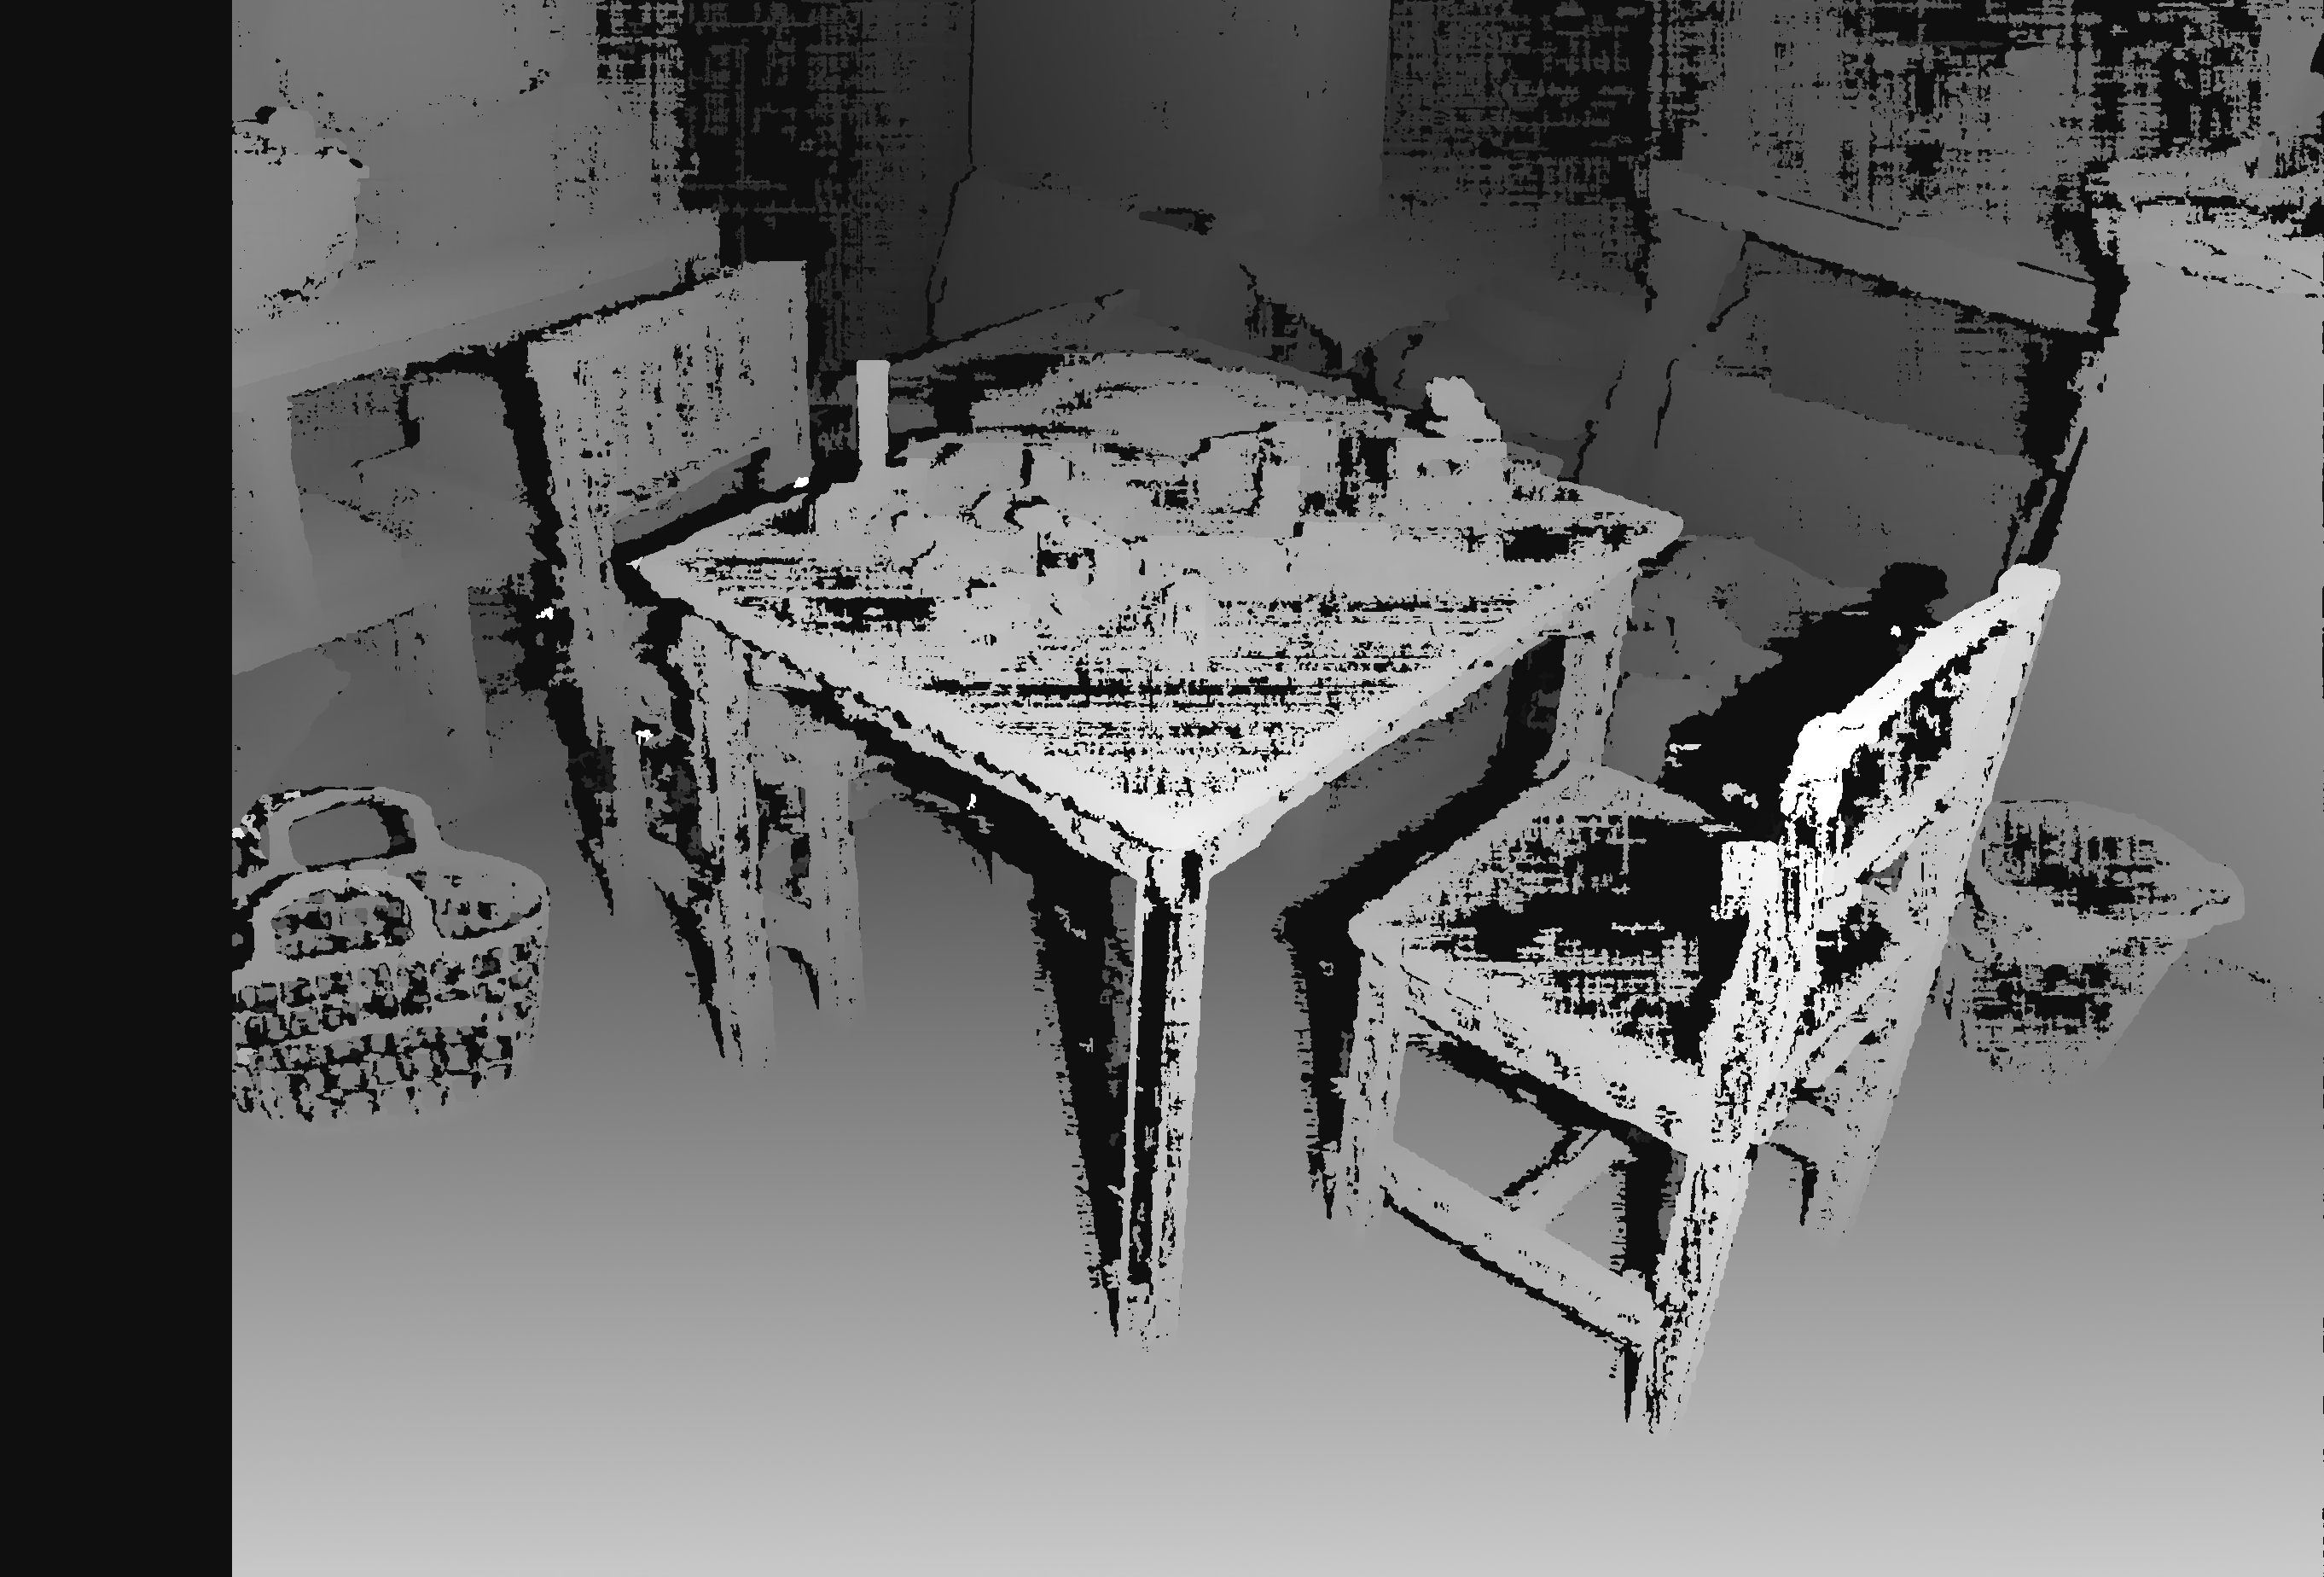
\includegraphics[width=0.8\textwidth, height= 5cm, keepaspectratio]{images/opencv-baseline-test-playtable.png}
 		 \label{fig:opencv-baseline-test-table}
}
\caption{Results of disparity images obtained with the disparity-based lightweight method, the SGM-based method and the baseline result from the OpenCV built-in method}
\label{fig:test-novel-methods-table-01}
\end{figure}

\begin{figure}[t]
	\centering
	\subfigure[Input left raw image ]{
 		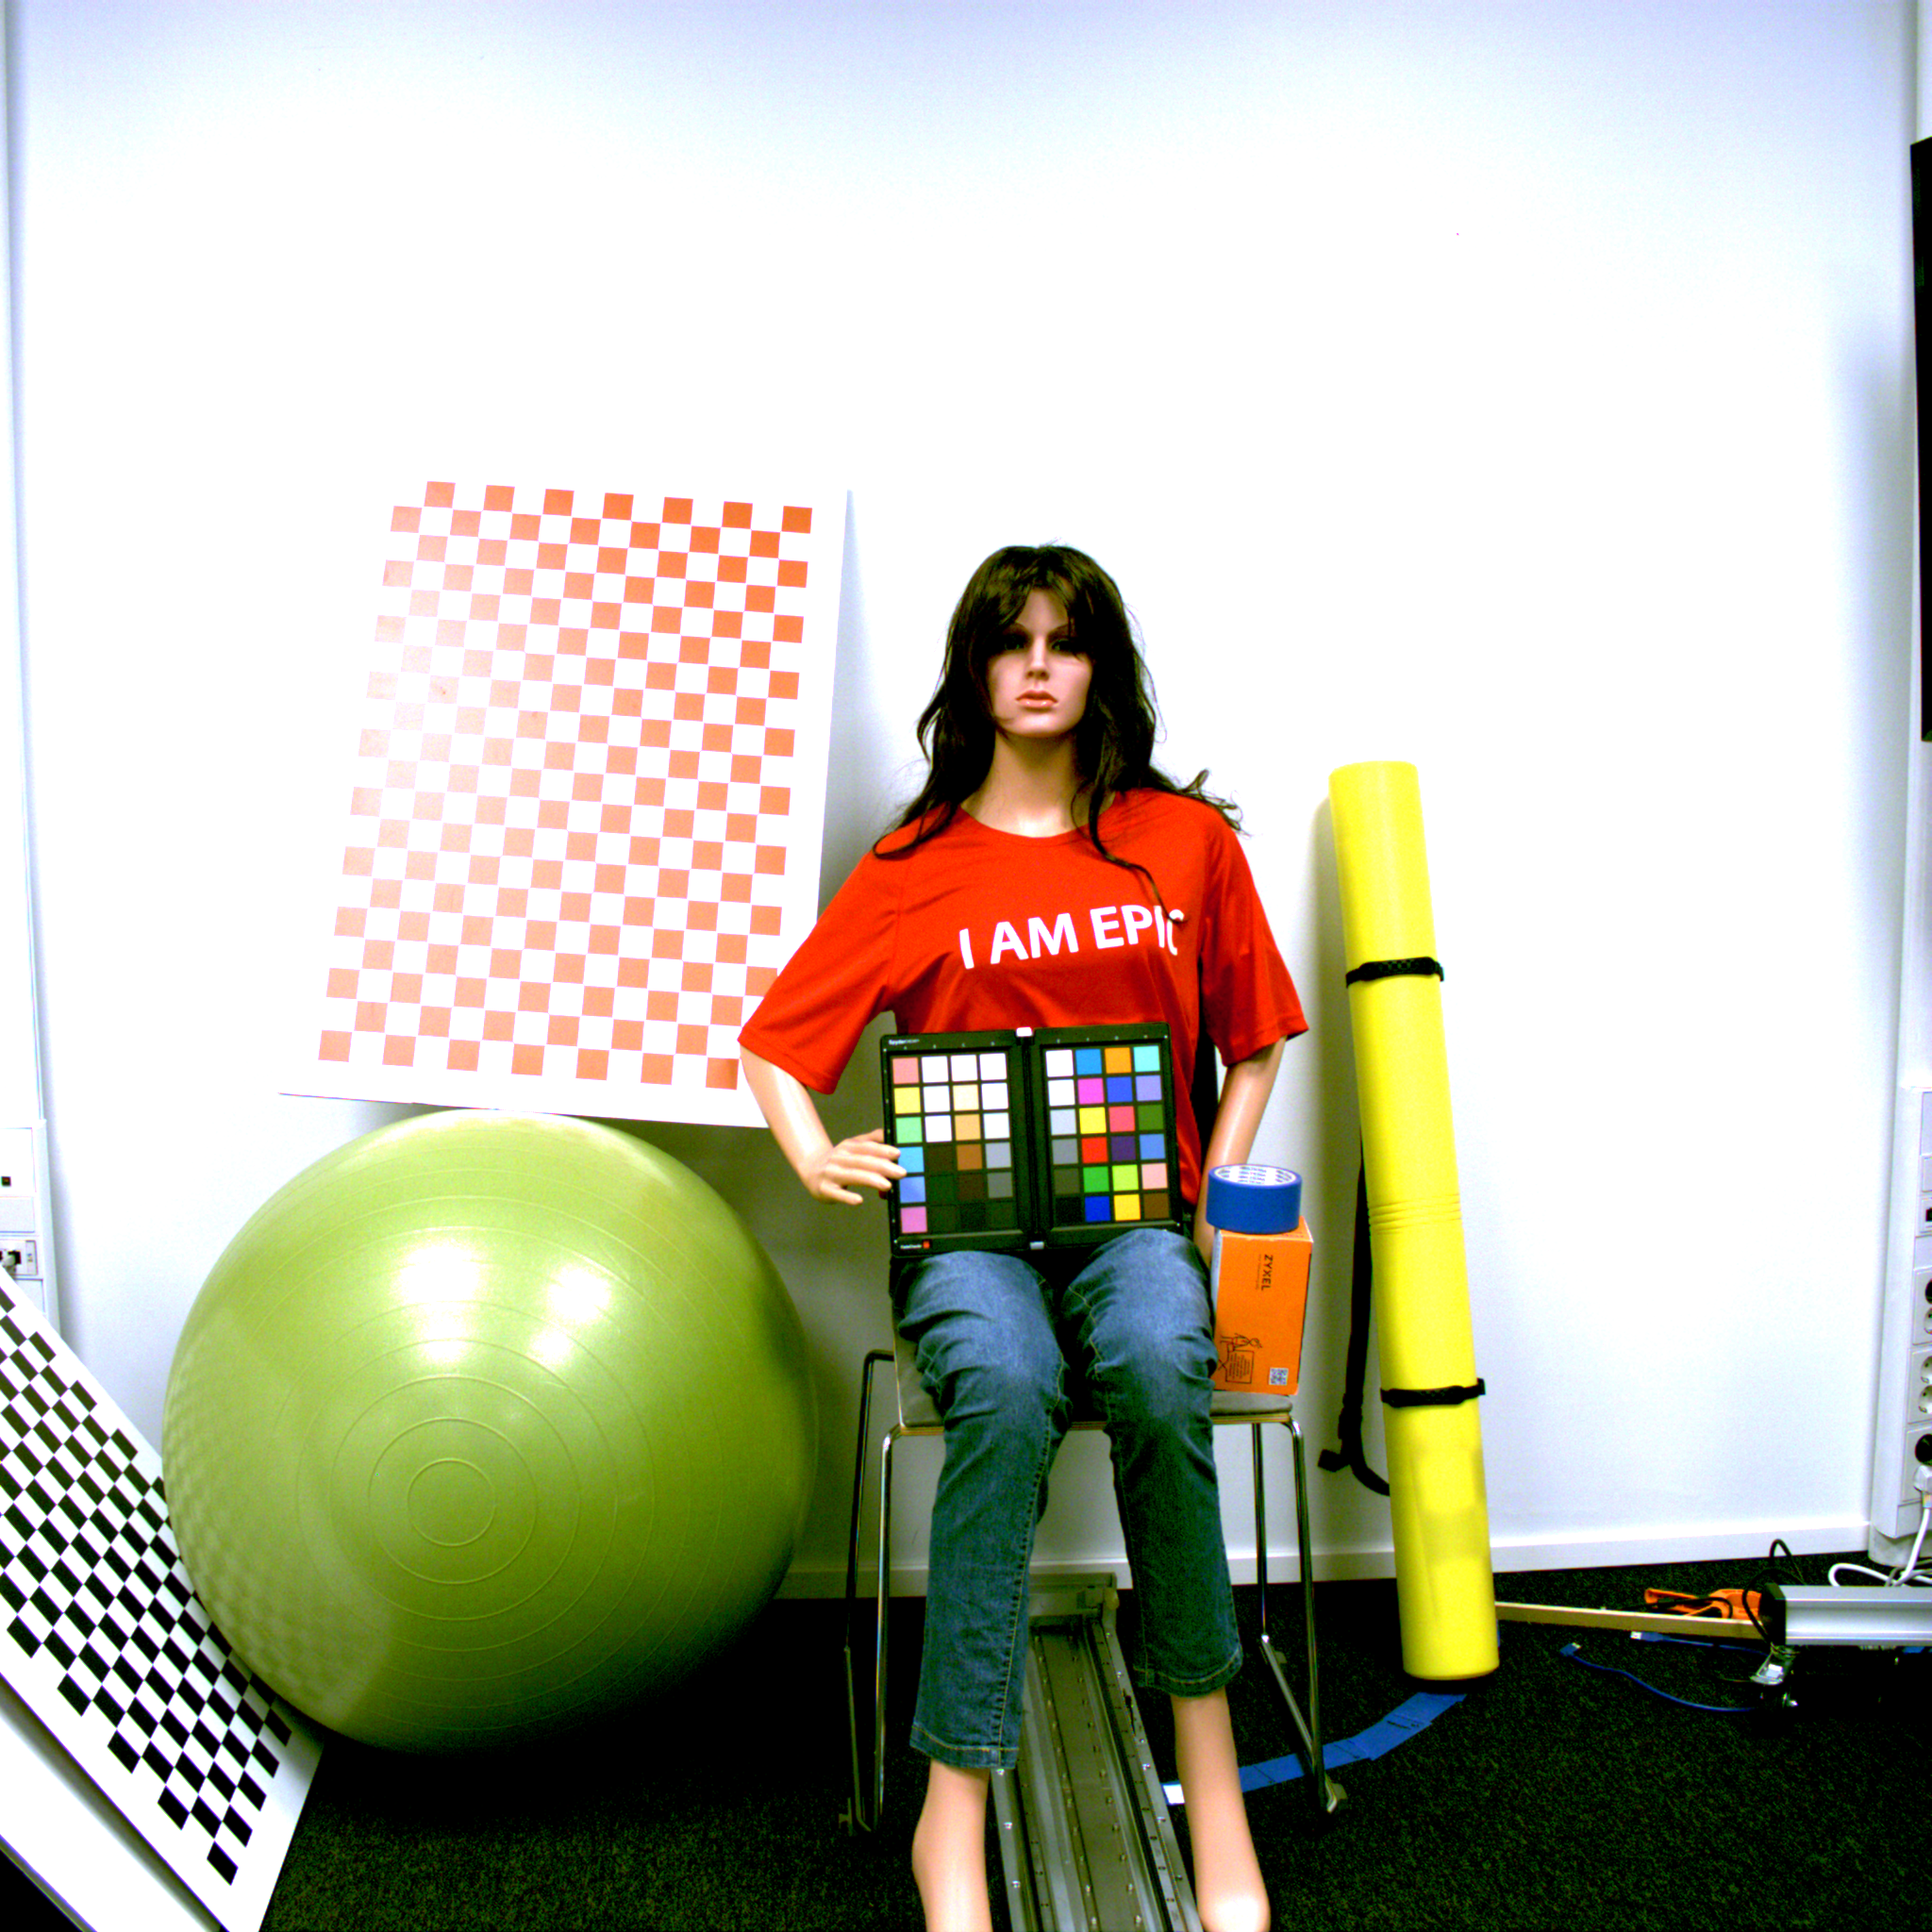
\includegraphics[width=0.4\textwidth, height= 5cm, keepaspectratio]{images/input-image-raw-left.png}
 		\label{fig:raw-image-4eye-der-method-left}
}
	\subfigure[Input right raw image]{
 		 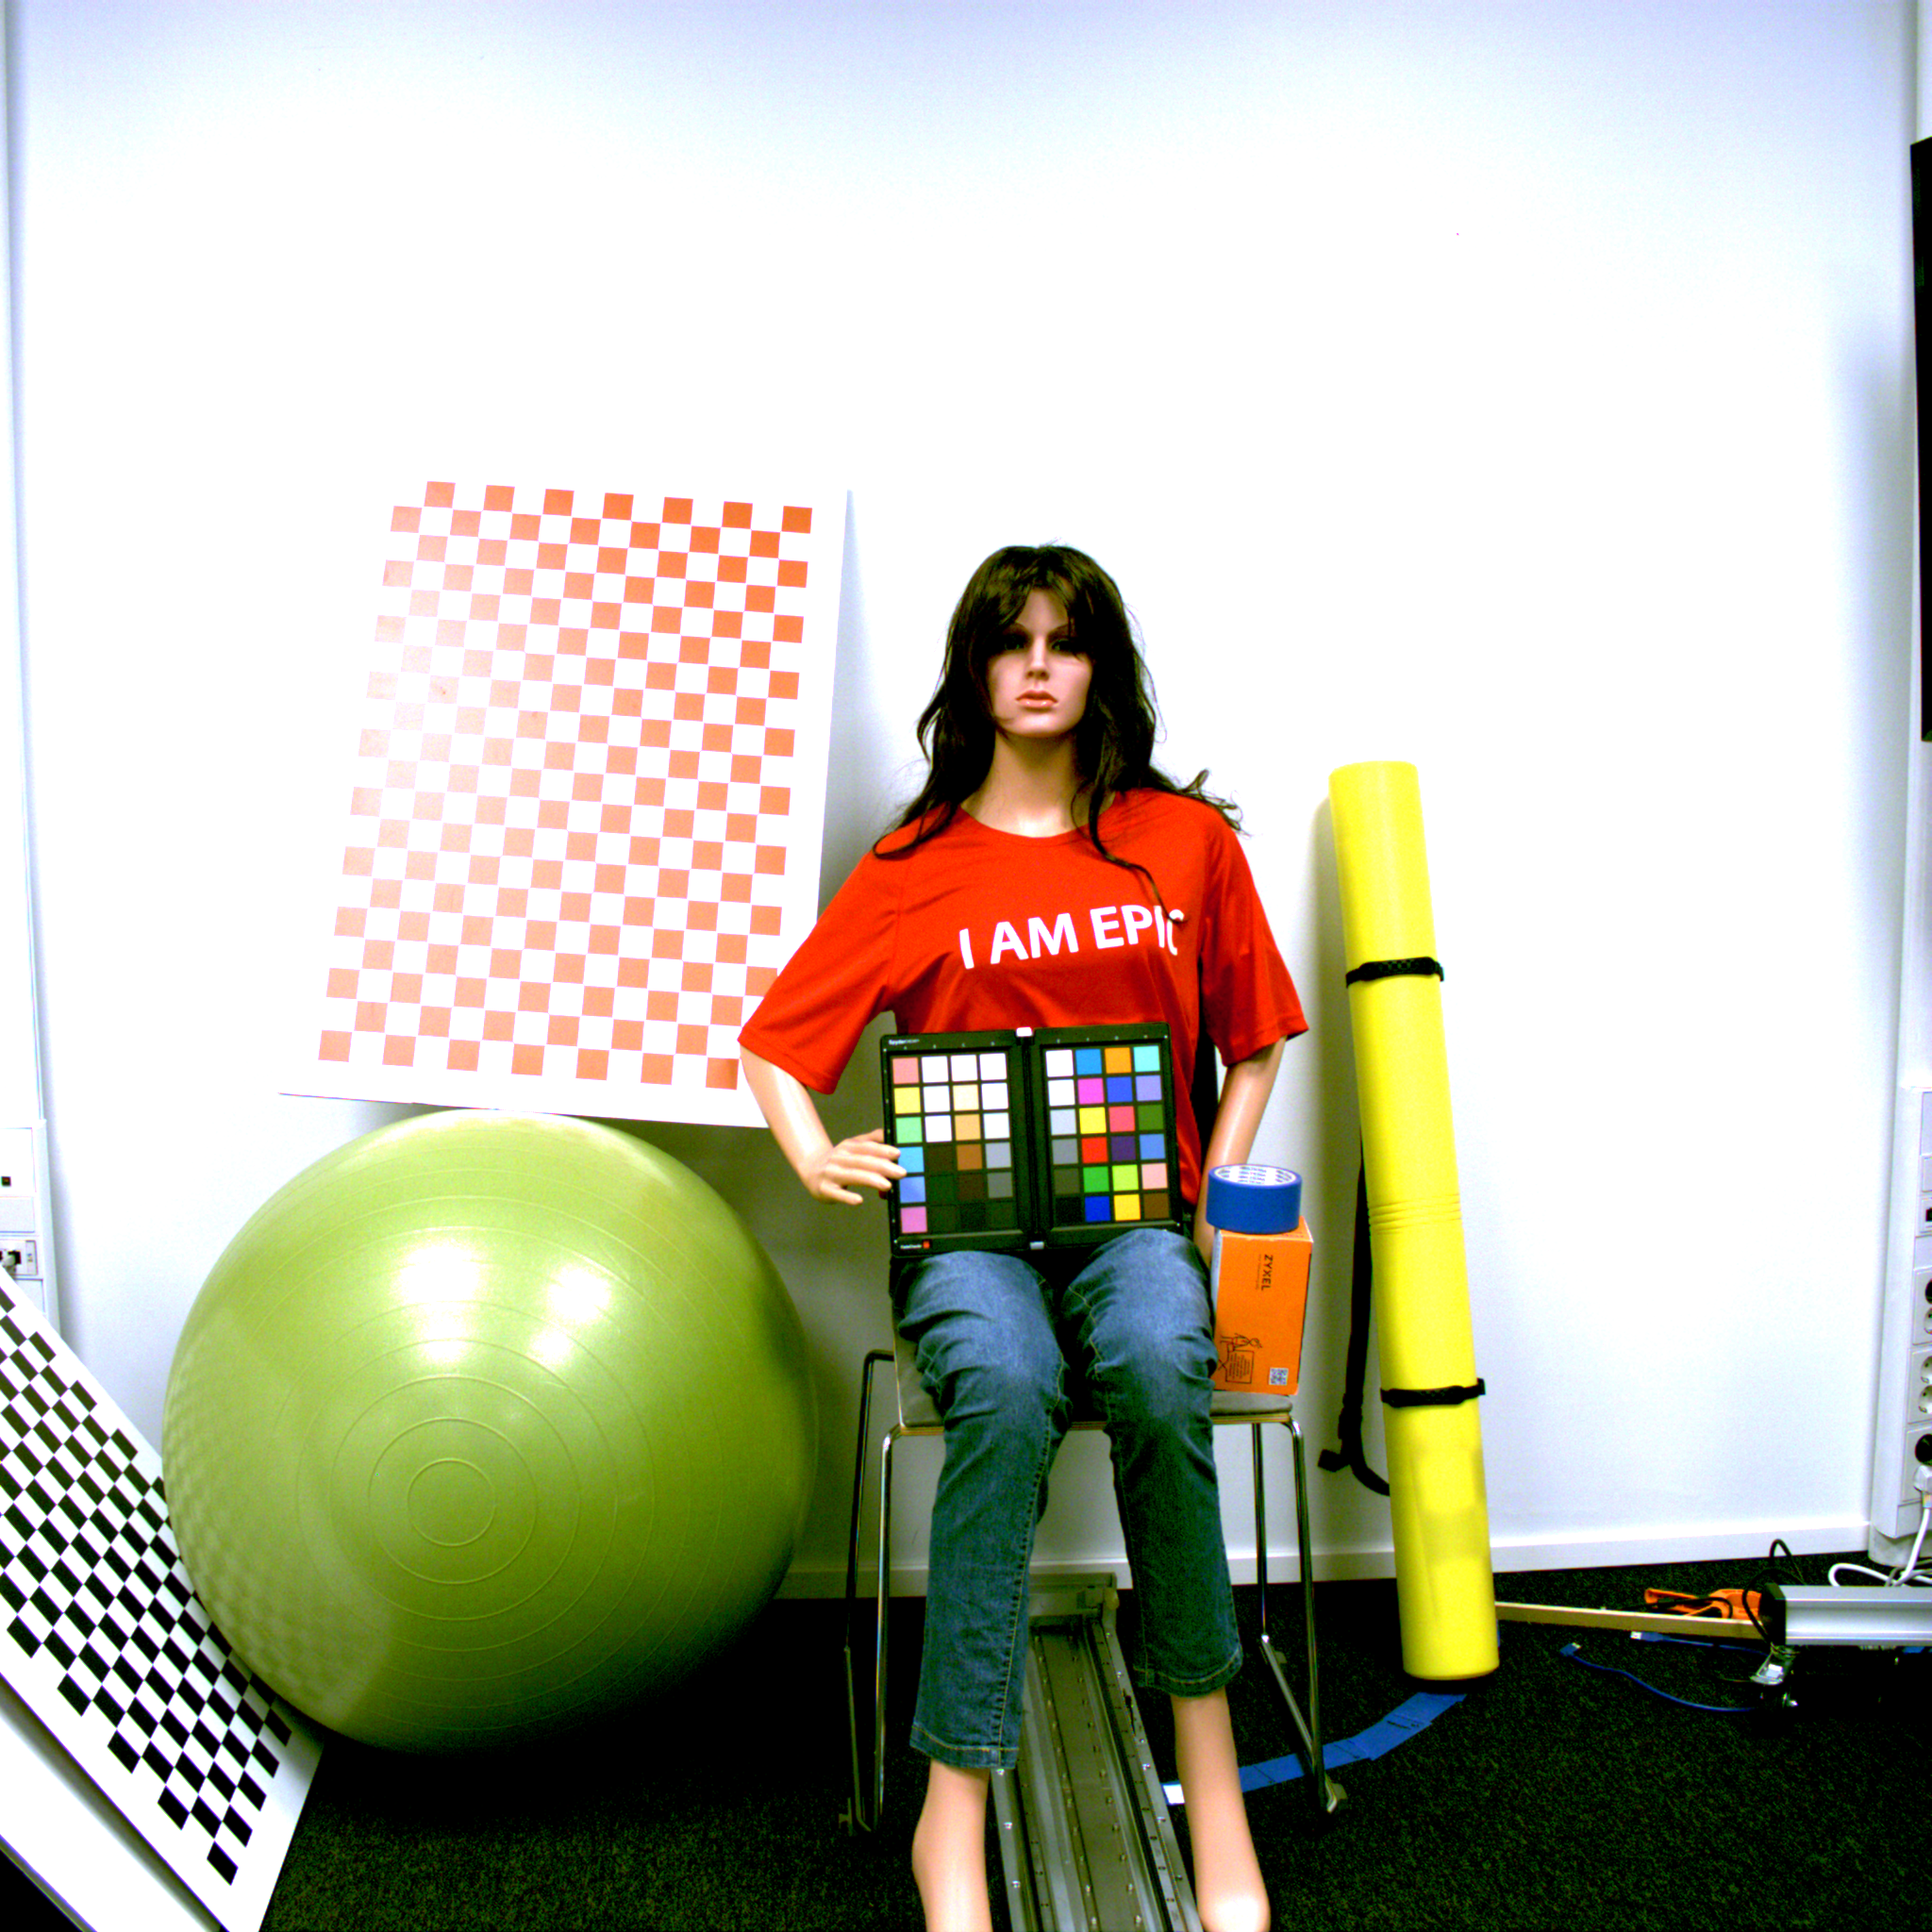
\includegraphics[width=0.4\textwidth, height= 5cm, keepaspectratio]{images/input-image-raw-right.png}
 		 \label{fig:raw-image-4eye-der-method-right}
}
	\subfigure[Input point cloud]{
	 	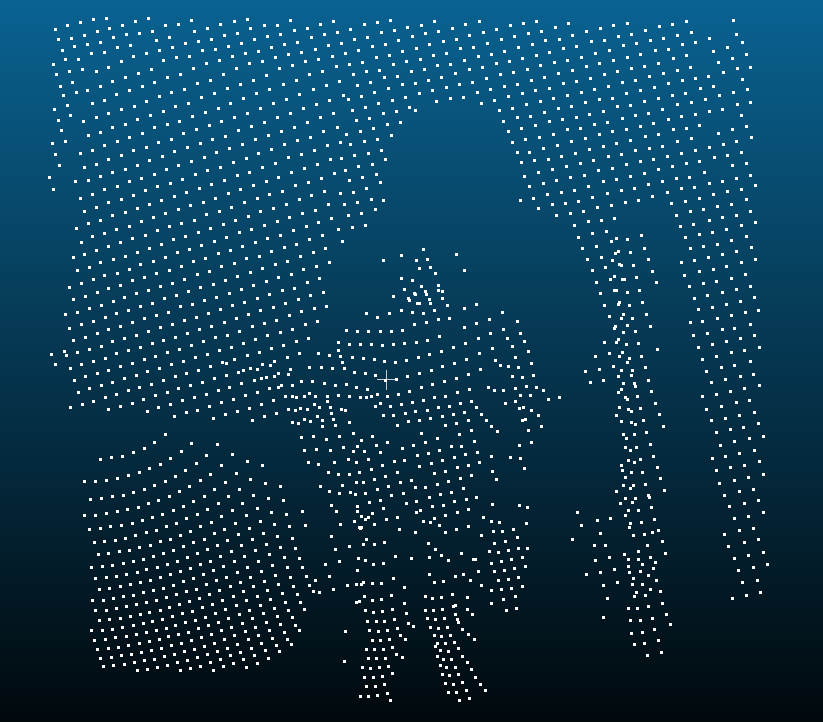
\includegraphics[width=0.4\textwidth, height= 5cm, keepaspectratio]{images/point-cloud-4eye-input.png}
 		\label{fig:input-point-cloud-4eye-der-method}
}
	\subfigure[Output dense point cloud]{
	 	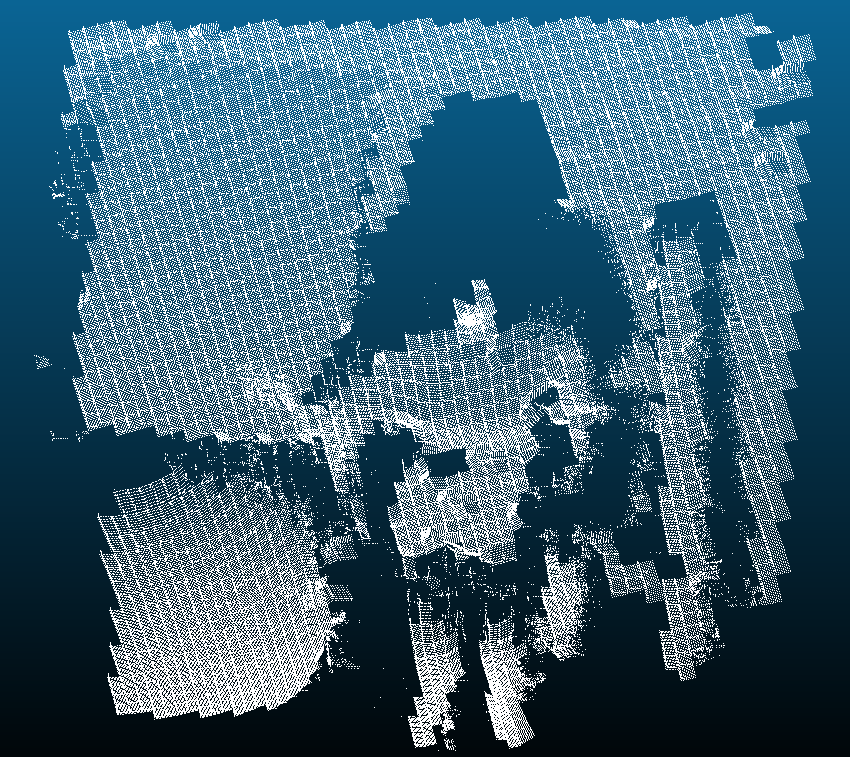
\includegraphics[width=0.4\textwidth, height= 5cm, keepaspectratio]{images/point-cloud-4eye-post-proc-median.png}
 		\label{fig:output-point-cloud-4eye-der-method}
}
\caption{Pair of raw images from the LaDiMo device, initial grid of point and final point cloud estimated with derivative-based method}
\label{fig:result-4eye-derivative-method}
\end{figure}

As Figure~\ref{fig:disparity-test-02} proved, it is possible to achieve reasonable results with the designed method.
However, the interesting thing is that, the initial tests performed show that, exploiting a sparse enough grid of points, which carry information on their 3D positions, the overall implementation can be made faster.\\
Therefore, after the initial researching phase, the algorithm started to be implemented in C++, in order to have a faster execution with respect to MATLAB, employing functions from the OpenCV library.
In this regard, Figure~\ref{fig:test-novel-methods-table-01} presents the grayscale disparity image achieved by applying the two designed methods, the derivative-based one and the SGM-based one, and then the outcome of the OpenCV built-in method is proposed as baseline for a visual comparison.\\
Therefore, considering the results of the disparity image of the \textit{Playtable} dataset, some thoughts can be formulated.
First of all, as expected, in the baseline result in Figure~\ref{fig:opencv-baseline-test-table} the object are more detailed.
This is, thus, highly visible where the object present small or thin features, as for the bag in the middle-left area of the image.
Moreover, with the OpenCV \texttt{stereoSGBM()} algorithm there is an higher accuracy for the regions close to edges. \\
However, it has to be pointed out that, even if the OpenCV method has a lower amount of \textit{local} noise, e.g. along the object edges, which are visibly clear, it is affected by higher amount of \textit{general} noise, especially in occluded or texture-less areas.
Regarding this detail, both of the results obtained with the designed algorithms present a lower accuracy along edges, highlighted by the \textit{hairy} contours, however the surfaces are in general smoother.
Let us consider the top of the table or of the chairs, or even the wall in the background, as an example.
In the results of Figures~\ref{fig:derivative-based-test-table} and \ref{fig:sgm-based-test-table} the black spots are not generated.
They are, most likely, due to the occlusions presents in the two stereo images, considering the table and the chairs, or they are generated in texture-less regions, as for the wall, for which it is known that the SGBM algorithm tends to fail.\\
More interesting results can be then visualized when taking into account the outcomes of the different algorithms obtained using images acquired by the company device.
As a matter of fact, in this case, contrarily to the images from widely-used datasets, such as the Middlebury 2014, the KITTI 2012 and KITTI 2015, there could likely be calibration errors in the stereo pair.
This leads to a mismatch between the epipolar lines of the two images, which should be overlapped to the image scanlines, when using a rectified stereo pair. 
Therefore, this problem causes a complete failure of the normal SGBM procedure, as Figure \textbf{reference bad sgm images} demonstrates.\\
On the other hand, the designed method, thanks to the information coming from the points grid, is able to recover from small mismatching errors.
This condition proves the suitability of such a method in various situations, making it appropriate for those situations in which errors, even if minimal, cannot be avoided. 
It is, in fact, well known that in most of the real environment conditions it is generally difficult to have stable and controlled conditions, especially for lighting and for the physical stability of the hardware. 
The latter requirement is then extremely important for the accuracy of the final result. 
For this reason, in every industrial and commercial device employed in 3D estimation, as could be LiDAR or standard camera based hardware, a strong attention is provided to the system setup. 
However, errors related to unpredictable events or to little software bugs can affect the further computations, which would exploit the device outcome. 

\subsection{Consistency check over derivative computation}
\label{subsection:result-consistency-check}

\begin{figure}[t]
	\centering
	\subfigure[Consistency check for derivative calculation]{
 		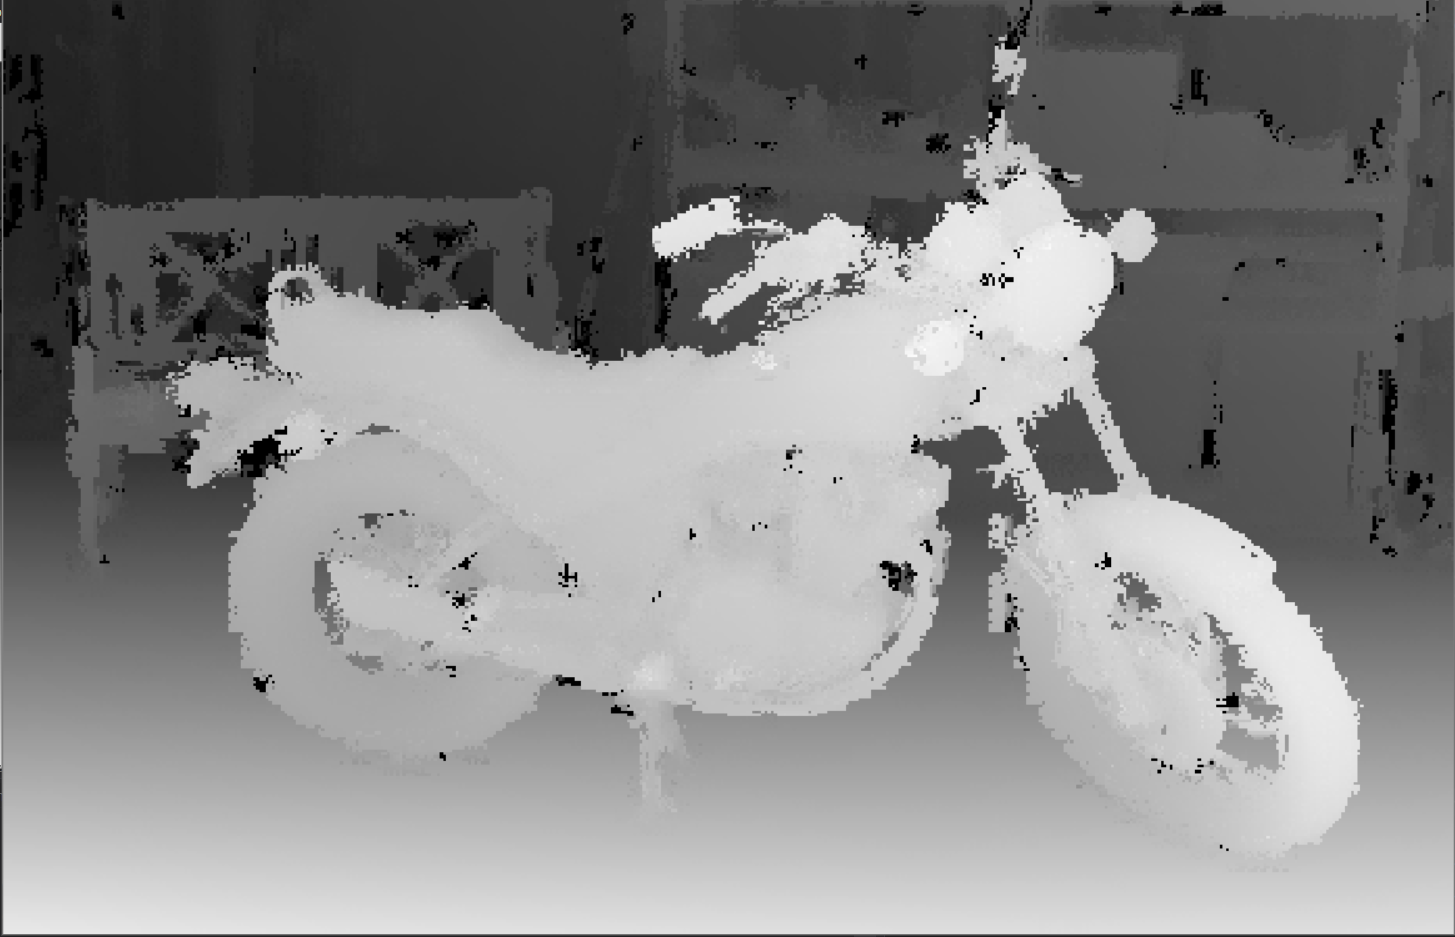
\includegraphics[width=0.4\textwidth, height= 5cm, keepaspectratio]{images/consistency-check-for-deriv-moto.png}
 		\label{fig:consistency-check-moto-01}
}
	\subfigure[No consistency check for derivative calculation]{
 		 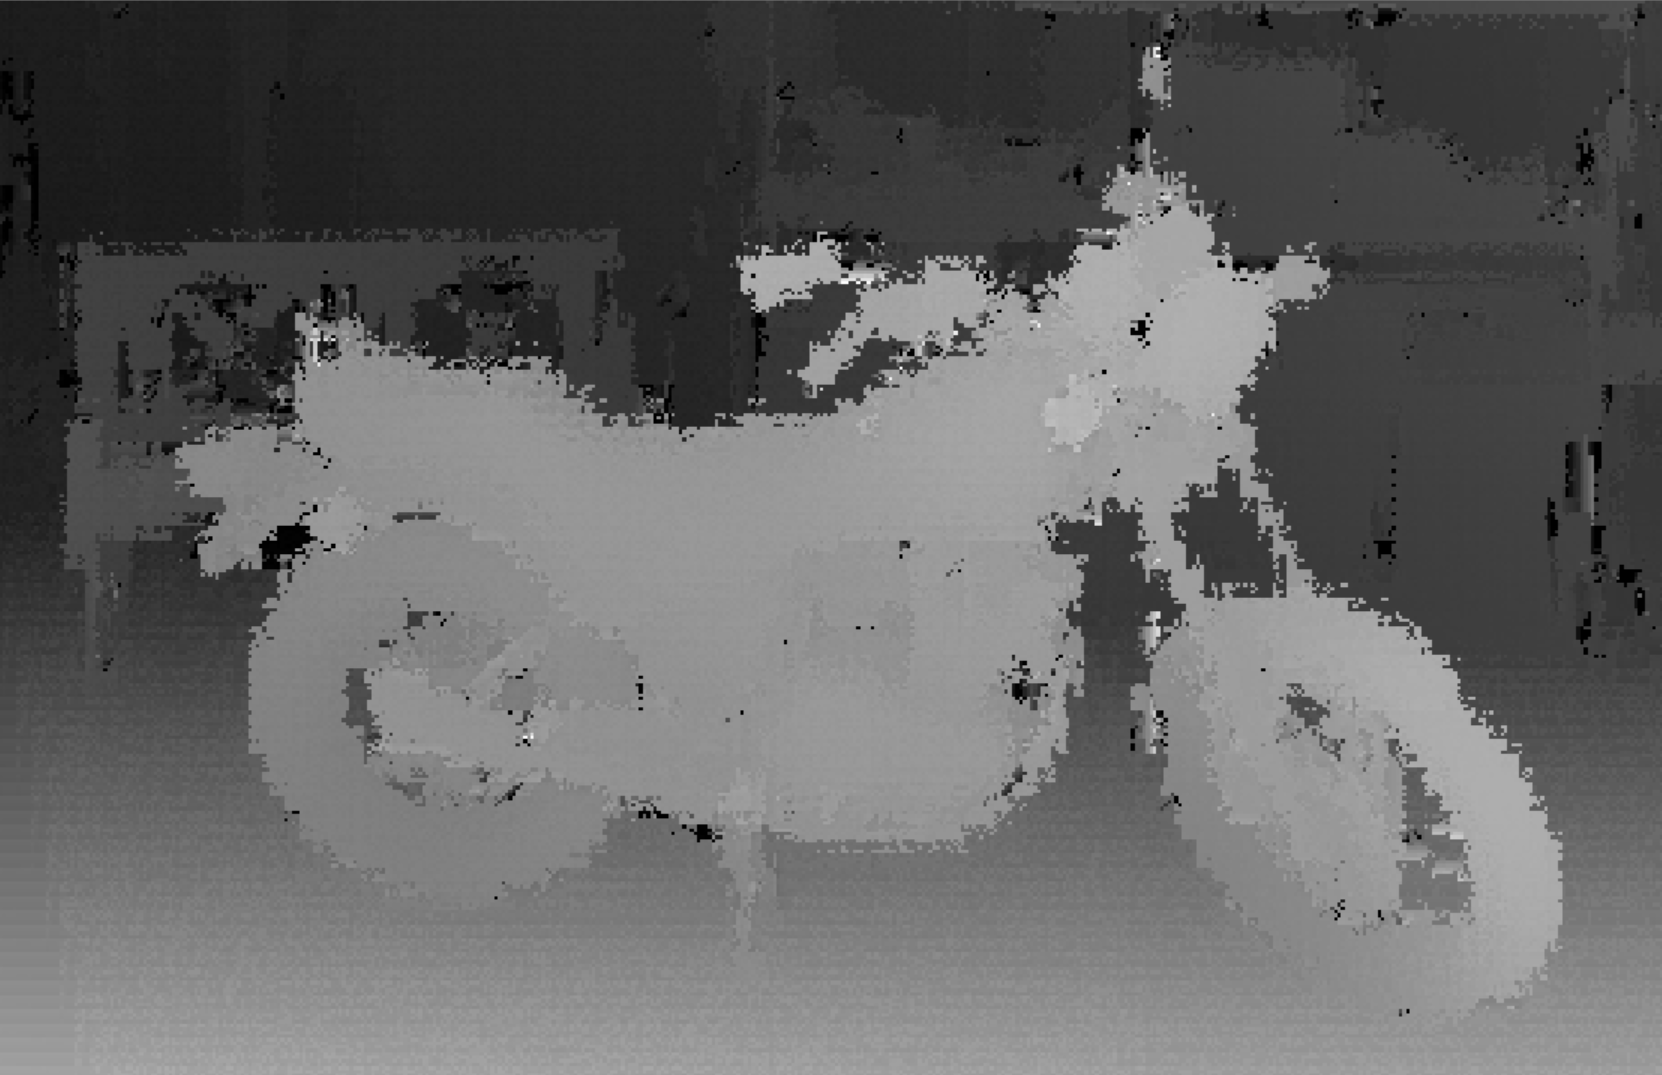
\includegraphics[width=0.4\textwidth, height= 5cm, keepaspectratio]{images/no-consistency-check-for-deriv-moto.png}
 		 \label{fig:no-consistency-check-moto-01}
}
\caption{Comparison between applying and not a consistency check procedure over the same image}
\label{fig:consistency-check-comparison-moto-01}
\end{figure}

During the algorithm designing a specific phase of the pipeline demonstrates to be extremely important. 
Specifically, it consists on the \textit{consistency check} performed during the derivative computation when running the algorithm exploiting the simulated grid of points.
Actually, this consistency check becomes relevant in proximity of the edges, where the magnitude of the $Z$ component of a derivative calculated between two points that belong to far objects, and thus cut by an occlusion, tends to explode.
Therefore, this will affect the estimation procedure, which will most likely carry out wrong values for the computations performed in those areas. \\
Figure~\ref{fig:consistency-check-comparison-moto-01} clearly demonstrate the difference on the final result when the consistency check over the derivatives calculations is applied or not.
When the magnitudes of the derivatives evaluated for a specific points are not correctly adjusted, if a set threshold on the $Z$ components of the derivative vector is exceeded, the final disparity image will show a huge amount of noise, which is obviously related to incorrect estimations.
Figure~\ref{fig:no-consistency-check-moto-01} is the proof of that.
Contrarily, in Figure~\ref{fig:consistency-check-moto-01} a better disparity map is visualized, which comes out when the consistency check operations are carried out.\\
Therefore, since the tests performed over the dataset images and using a simulated point grid, the necessity of the derivative correction was proven to be a valuable, and yet fundamental, step to reach an accurate result.

\subsection{Different thresholds for edge intensity result comparison}
\label{subsection:soft-strong-edge-threshold}

\begin{figure}[t]
	\centering
	\subfigure[Utilization of unique threshold over the whole input grid]{
 		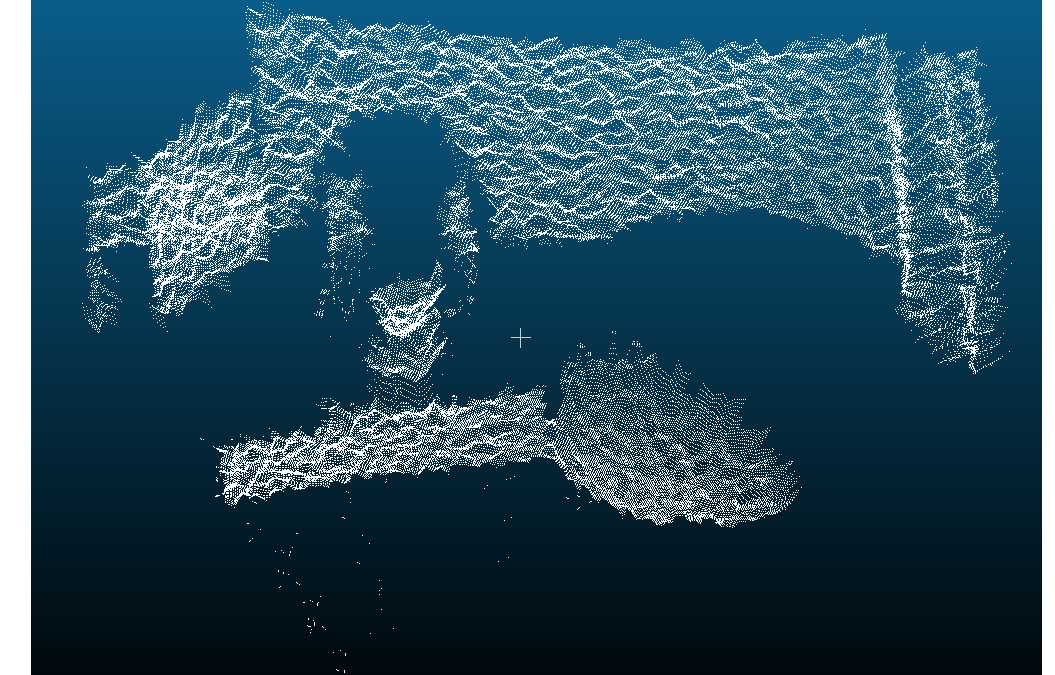
\includegraphics[width=0.4\textwidth, height= 5cm, keepaspectratio]{images/micro-device-result-no-double-threshold-edges.png}
 		\label{fig:single-threshold-micro-01}
}
	\subfigure[Utilization of multiple threshold for distinguish edge strength]{
 		 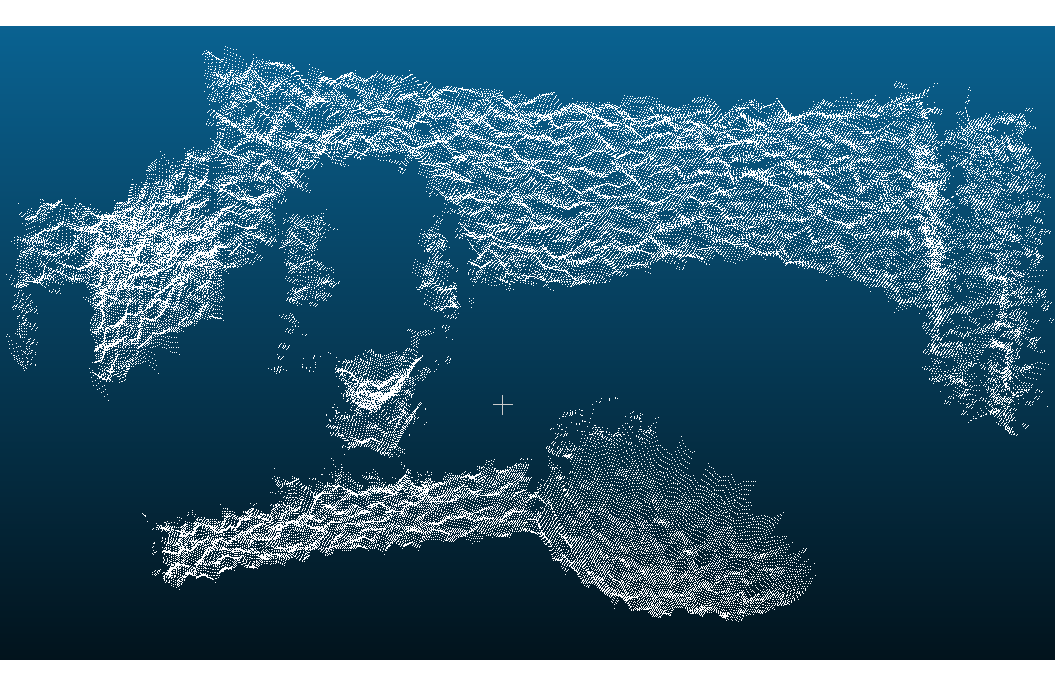
\includegraphics[width=0.4\textwidth, height= 5cm, keepaspectratio]{images/micro-device-result-yes-double-threshold-edges.png}
 		 \label{fig:multiple-threshold-micro-01}
}
\caption{Comparison between utilization of different thresholds distinguish edge strength}
\label{fig:threshold-soft-strong-edges-micro-01}
\end{figure}

Taking into account the results obtained employing the company device, some considerations can be performed in relation to useful improvements that have been implemented to the algorithm during its development. \\
A modification to the initial pipeline of the algorithm, which shows to give interesting improvement in the accuracy of the final 3D point cloud estimated, stands in the utilization of multiple threshold for the edge analysis.
Specifically, as visible in Figure~\ref{fig:single-threshold-micro-01}, utilizing a unique threshold for edge checking over the whole input cloud wrong estimations are generated.
These are depicted in Figure~\ref{fig:single-threshold-micro-01} by the outlier points and are particularly visible where there is not a strong difference in depth among neighbouring point, as it happens between the face of the statue and calibration board on the foreground.\\
On the contrary, when different cases have been implemented in relation to different types of edges, strong and soft, those outliers have gone away, as Figure~\ref{fig:multiple-threshold-micro-01} depicts.


\section{Stereo-matching based method results}
\label{section:stereo-match-results}

Taking into account the results obtained from this method it has to be said that they does not reflect the optimal trade-off compared to the derivative-based algorithm.
As a matter of fact, the computational time of this algorithm is actually relatively long. 
Despite that, the point cloud obtained in output is really dense, as expected, being the algorithm based on pixel-wise computations. 
However, if the results among all the analysed approaches are compared, this increase in density is not worth the rise in computational time, thing that would probably make this method intractable for real time applications.
A real time execution of this approach could be, after all, reached with a proper GPU implementation and setting up a wise construction of the pipeline.
Besides that, its best application could be most likely implied for use cases that need a high level of accuracy by sacrificing proper real time performance.\\
Therefore, the principal comparison could be done between the derivative-based approach, which can be described as a lightweight method, and the standard SGBM method built in OpenCV.


\section{OpenCV method baseline results}
\label{section:opencv-baseline-results}

Comparing the designed lightweight method and the built-in OpenCV SGM-based \texttt{stereoSGBM()} algorithm the following considerations can be provided.\\
First of all, with database images that are taken under optimal conditions and properly adjusted the OpenCV function results to be more accurate and it outputs a more correct disparity map.
The downside is that, it is relatively computationally expensive, at least when executed on a normal laptop exploiting only the CPU.\\
On the other hand, the developed algorithm comes out to be sensibly faster, if run on the same machine and in the same conditions. 
At the same time, it is less accurate, though. 
Regarding that, it has to be underlined that its computation is not optimized.
Moreover, only basic pre and post-processing operations have been applied to its pipeline.
Therefore, it could provide most likely better and more accurate results and probably even in a faster time. \\
Furthermore, an important achievement stands on the use of the initial grid of sparse points.
As a matter of fact, it allows to recover from calibration errors and noise, which are almost unavoidable when images are taken in a real environment under normal conditions.  
Additionally, the input grid helps to deal with texture-less regions of the specific scene, which tend to make the normal SGM method fail. \\
Therefore, at this stage of the work the result obtained with the derivative based method cannot be considered as optimal and the algorithm itself need some further work in order to be considered as competitive in the market, guaranteeing the level of accuracy necessary for providing safety in a real world application.
Nevertheless, the implementation done until this point and the tests accomplished showed that improvements can be provided to reach a high level of accuracy in the estimation, while keeping the computational time in a range suitable for real-time applications. \\
Now, a final overall comparison among the results obtained with all the methods will follow in the next section. 
Some last comments about the achieved outcomes and their suitability are going to be outlined. \\
In conclusion, a final discussion over the overall work is going to be proposed in Chapter~\ref{chapter:discussion}, where considerations about further improvements will be delineated. 
 
\section{Overall comparison of the outcomes}
\label{section:method-comparison}

Summing up the outcomes obtained and the theoretical capabilities of all the different methods studied, the results of the derivative-based method can be considered as accurate result for the purposes of a researching project.
Obviously, when compared over perfect dataset images with properly optimized methods, as the \texttt{stereoSGBM()} available in the OpenCV libraries, a certain lack in accuracy is visible.\\
However, some important features of the designed method, which highlight its potential suitability for real-time computer vision based applications, can be pointed out by analysing the outcomes achieved.
Firstly, a key component of that method is the input grid of sparsified points, which allows to make accurate estimations over all the scene and recover from small calibration errors.
Moreover, that feature supports the possibility of getting accurate results even in texture-less areas of the scene, which are extremely challenging for pure stereo matching based methods.
As a matter of fact, in the literature studied, that was a problem that many researchers tried to overcome in multiple ways, such as designing deep learning based algorithm in the latest years.
In those publications, impressive results have been obtained by improving a standard SGM-based routine with convolutional neural networks.
However, even if they outperforms almost all the previous algorithms, that performance is reached over standard dataset images, such as the Middlebury 2014, KITTI 2012, KITTI 2015 and over synthetic datasets.
Those datasets obviously cover a massive number of real world situations, yet, it would be always possible to deal with environments for which the network has not been properly trained. \\  
Therefore, another core feature of the designed algorithm stands exactly on that.
It can be employed in every kind of scene and it does not need any type of pre-training.
Thus, once it has been embedded in a stereo device, and adjusting the parameters relatively to the hardware specifications, it can provide a dense and accurate 3D point cloud of the scanned scene with a potential real-time performance.
